While modeling the Dark Ages is quite feasible given a few simple parameters and initial
coniditions set by the CMB, developing an accurate model of the EoR is quite difficult
to do given its non-linear nature. A picture of reionization has unfolded
giving us some insight into how reionization progressed. When the first luminous sources formed from graviational collapse of
overdense regions, they began producing UV photons which ionized the neutral gas in the
IGM immediately around them. This ionized gas, now transparent to UV radiation,
formed ``bubbles'' of material around these early galaxies. As these sources grew and others formed, ionizing radiation
continued to pour into the IGM, causing these bubbles to grow and overlap with ionized
bubbles surrounding neighboring sources. This progressed until all bubbles surrounding these
early sources overlapped, leaving only trace amounts of neutral hydrogen within galaxies.
This complete ionization of hydrogen in the IGM is what marked the end of reionization.

This general picture of reionization is relatively well accepted, but the details
are largely unconstrained and leave many questions unanswered.
The beginning of reionization, the time it took the first luminous sources to fully ionize
the IGM, and size and growth rate of early ionized bubbles are open questions which are
sought to be answered. If we are able to answer these questions, we also have the
ability to shed light on more fundamental areas of astrophysics, such as what the
first luminous objects were like and how they formed.

While current measurements of the EoR are slim, there are a few studies that allow us
to constrain the progress of reionization. Measurements of the polarization
of the CMB can help place some restriction on the timing of reionization. By assuming
reionization was instantaneous, the WMAP and Planck CMB probes used the optical depth of the
CMB to infer a reionization redshift of $z \approx 8.8$. In addition, high-redshift quasar studies provide insight to
when reionization likely came to a close. Using observations of the Gunn-Peterson trough, \cite{2006AJ....132..117F}
found that reionization concluded no later than $z \approx 6$. This technique will
be used in future experiments, namely with the James Webb Space Telescope, to further
constrain the neutral fraction of the IGM across cosmic time. The most up to date constraints on reionization including
Planck and high-redshift galaxy measurements can be found in Figure \ref{fig:reionization_constraints}.

\begin{figure}[th]
	\centering
	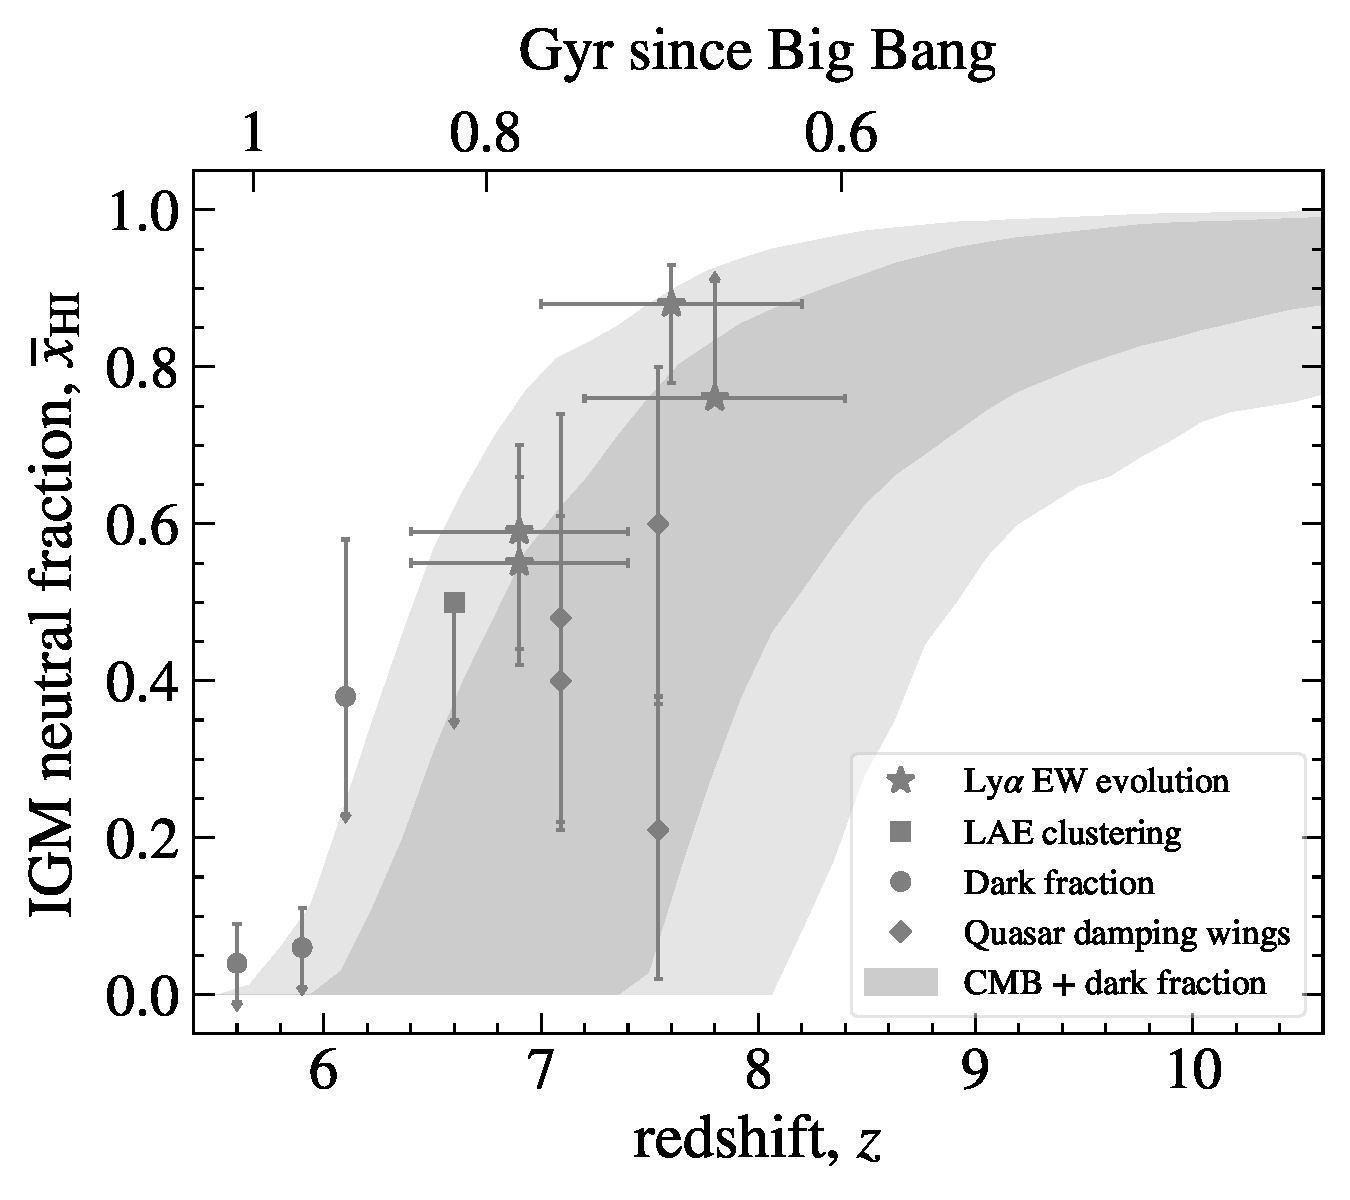
\includegraphics[width=0.7\textwidth]{tyler_reionization_history.pdf}
	\caption[Reionization Constraints]{Constraints on reionization. Modified from \cite{2019arXiv191103499W}}
	\label{fig:reionization_constraints}
\end{figure}


\begin{figure}[th]
	\centering
	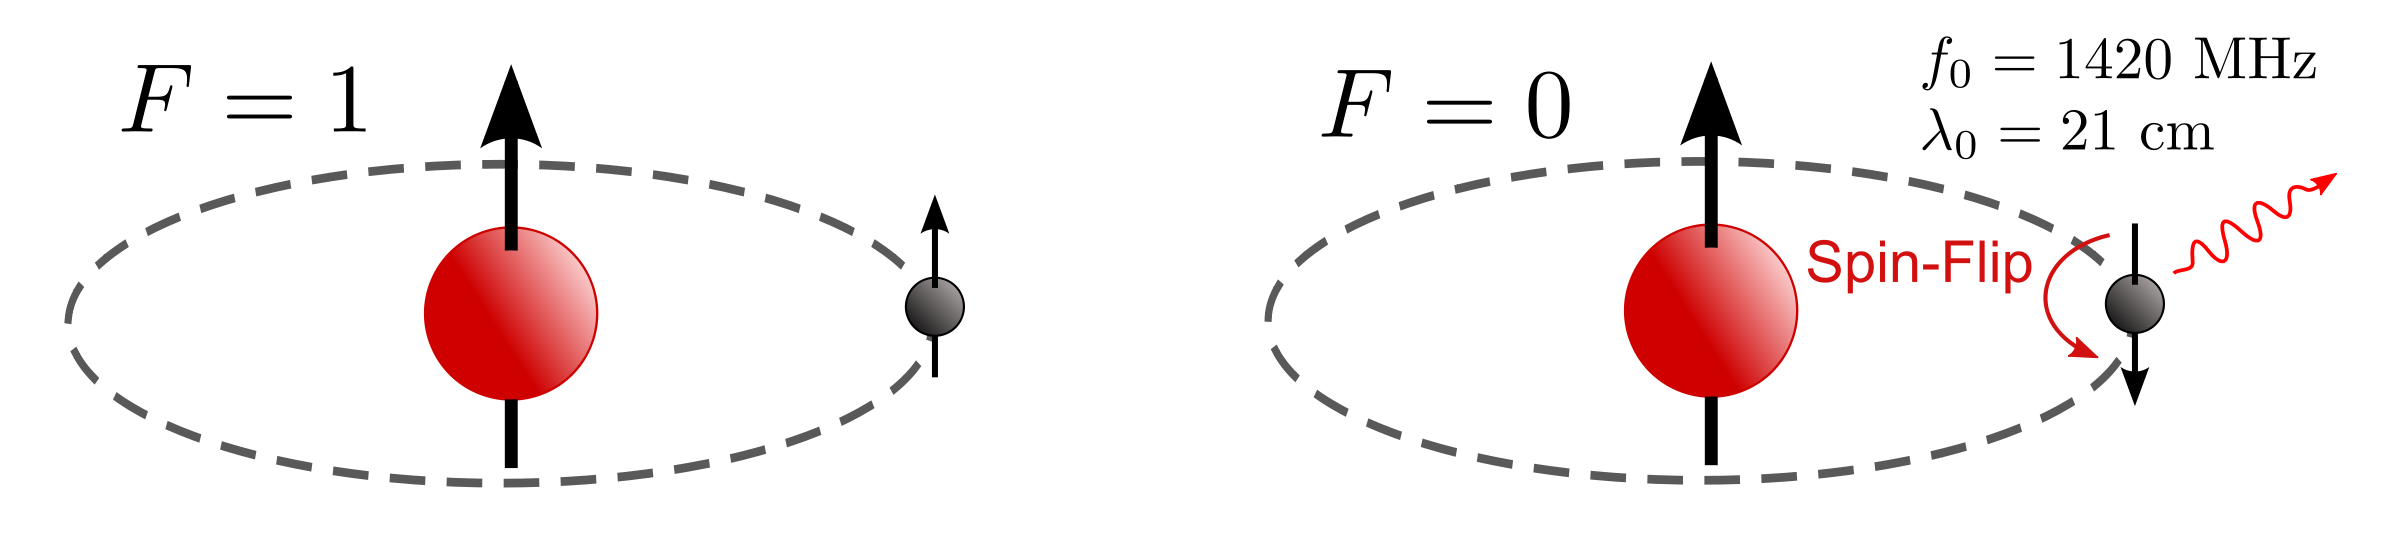
\includegraphics[width=0.90\textwidth]{spin_flip_H.png}
	\caption[Spin-Flip Transition of Neutral Hydrogen]{A depiction of the spin-flip transition of neutral hydrogen. Initially,
																					 the spin of the proton and electron are parallel and oriented
																					 in the same direction. The transition occurs when the electron's spin spontaneously
																					 flips from the higher energy parallel alignment to the lower energy anti-parallel alignment,
																					 releasing a photon with a wavelength of 21\,cm.}
	\label{fig:spin_flip}
\end{figure}

In addition to CMB and high-redshift quasar measurements, other techniques are being
developed to understand the progression of reionization. In particular, spectral line
intensity mapping looks to be promising method of studying the EoR by constructing
three dimensional maps of the universe using well-known spectral lines
(\hyperref[fig:spin_flip]{21\,cm}, \lya, CII, CO, etc.). The major advantage
of this method is that these spectral lines are narrow and well understood so observed redshift
maps directly translate to an observation of a specific cosmic time. This
method promises to place some of the tightest constraints on reionization by capturing
the behavior of the first luminous objects and the IGM on large scales.

\begin{figure}[th]
	\centering
	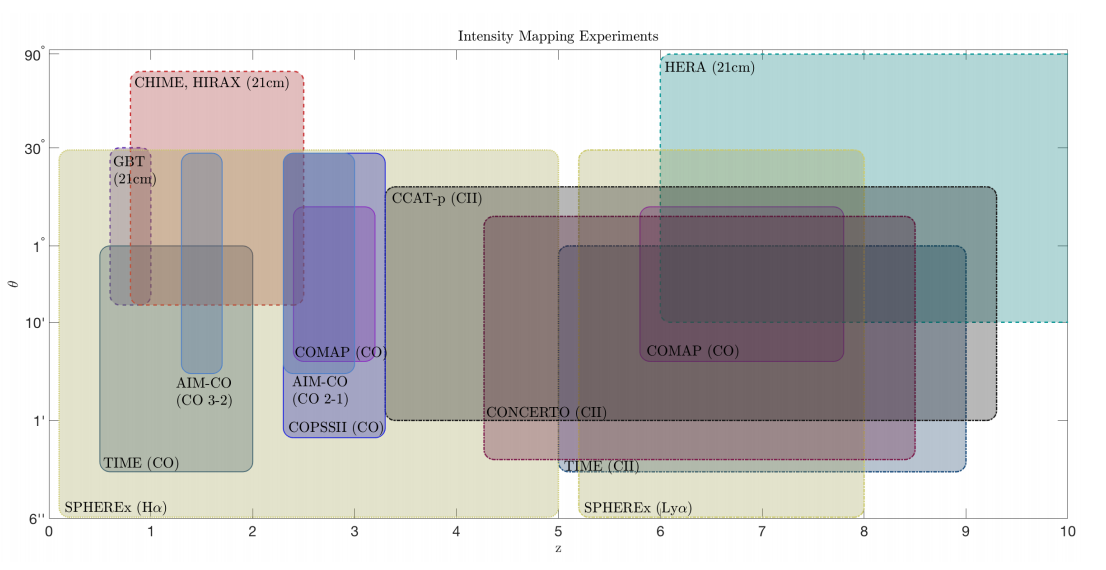
\includegraphics[width=0.95\textwidth]{results/intensity_mapping.png}
	\caption[Redshift and Resolution Coverage of Intensity Mapping Experiments]{A figure
					representing the resolution, field of view, and redshift range of upcoming intensity mapping
					experiments.}
	\label{fig:intensity_mapping}
\end{figure}
